\clearpage
\chapter{Special Triangles}
Special triangles are something you likely looked at back in geometry. However, they will serve a fundamental role in the next chapter when I talk about the unit circle. The two I'll look at in this chapter are the 30-60-90 and the 45-45-90 triangles. Special triangles are called "special triangles" because they're easy to solve for. The ratios for all the sides and angles are known. So, if you have one (side or angle) you have all of them.

The numbers in the names of these triangles refers to the values of the three angles. I'll begin with the 30-60-90 triangle and continue with the 45-45-90.
\section{The 30-60-90 Triangle}
The 30-60-90 triangle is a right triangle that has one angle of $30\degree$, one angle of $60\degree$, and a right angle ($90\degree$).
\begin{center}
    \begin{minipage}[c]{0.45\linewidth}
        \centering
        \captionof{figure}{30-60-90 Triangle}
        \label{fig:30-60-90}
        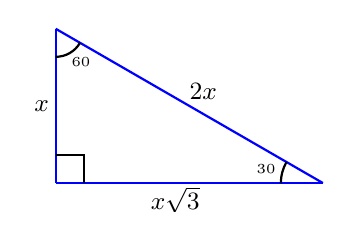
\begin{tikzpicture}
            \begin{axis}[
                xmin = -10, xmax = 100,
                ymin = -10, ymax = 100,
                height = 5.5cm, width = 5.5cm,
                axis lines = none%
            ]
                %Triangle
                \draw[color = blue, thick] (0,0) -- (0,55);
                \draw[color = blue, thick] (0,55) -- ({55 / tan(30)}, 0);
                \draw[color = blue, thick] (0,0) -- ({55 / tan(30)}, 0);

            % 30 Degree Angle
            \node[font = \tiny] at (75, 5) {$30\degree$};
            \draw[color = black, thick] ({(55 / tan(30)) - 15},0) arc (180:150:15);

            % 60 Degree Angle
            \node[font = \tiny] at (9,43) {$60\degree$};
            \draw[color = black, thick] (0, {55-10}) arc (270:330:10);

            %Side Labels
            \node[font = \small] at (-5, {55 / 2}) {$x$};                                   % x label 
            \node[font = \small] at ({55 / (2 * tan(30)) - 5}, -6) {$x\sqrt{3}$};           % xsqrt(3) label
            \node[font = \small] at ({55 / (2 * tan(30)) + 5}, {(55 / 2) + 5}) {$2x$};     % 2x label

            % Right angle symbol
            \draw[thick, color = black] (0,10) -- (10,10) -- (10,0);
            \end{axis}
        \end{tikzpicture}
    \end{minipage}
    \begin{minipage}[c]{0.50\linewidth}
        Regardless of the size and orientation of a 30-60-90 triangle, the side proportions and angle measurements will remain the same. When comparing to the short leg (vertical), the other leg is longer by a factor of $\sqrt{3}$ and the hypotenuse by $2$.\\\\Also note that the smaller leg is opposite the smaller angle!!
    \end{minipage}
\end{center}
\clearpage
You may also see this triangle depicted as having a short leg of length $1$, a long leg of length $\sqrt{3}$, and a hypotenuse of length $2$. It's exactly the same as the one shown in Figure \ref{fig:30-60-90}. It just has $x$ set equal to $1$.

\section{The 45-45-90 Triangle}
The 45-45-90 triangle is a right triangle that has two angles of $45\degree$ and a right angle ($90\degree$).
\begin{center}
    \begin{minipage}[c]{0.45\linewidth}
        \centering
        \captionof{figure}{45-45-90 Triangle}
        \label{fig:45-45-90}
        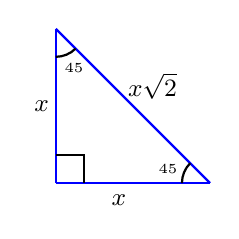
\begin{tikzpicture}
            \begin{axis}[
                xmin = -10, xmax = 100,
                ymin = -10, ymax = 100,
                height = 5.5cm, width = 5.5cm,
                axis lines = none%
            ]
            %Triangle
            \draw[color = blue, thick] (0,0) -- (0,55);
            \draw[color = blue, thick] (0,55) -- ({55 / tan(45)}, 0);
            \draw[color = blue, thick] (0,0) -- ({55 / tan(45)}, 0);

            % 30 Degree Angle
            \node[font = \tiny] at (40,5) {$45\degree$};
            \draw[color = black, thick] ({(55 / tan(45)) - 10},0) arc (180:135:10);

            % 60 Degree Angle
            \node[font = \tiny] at (6.5,41) {$45\degree$};
            \draw[color = black, thick] (0, {55-10}) arc (270:315:10);

            %Side Labels
            \node[font = \small] at (-5, {55 / 2}) {$x$};                                       % x label 
            \node[font = \small] at ({55 / (2 * tan(45)) - 5}, -6) {$x$};                       % xsqrt(3) label
            \node[font = \small] at ({55 / (2 * tan(45)) + 7}, {(55 / 2) + 7}) {$x\sqrt{2}$};   % 2x label

            % Right angle symbol
            \draw[thick, color = black] (0,10) -- (10,10) -- (10,0);
            \end{axis}
        \end{tikzpicture}
    \end{minipage}
    \begin{minipage}[c]{0.50\linewidth}
        Figure \ref{fig:45-45-90} shows a 45-45-90 triangle with all of the sides labeled. Regardless of the size and orientation of a 45-45-90 triangle, the side proportions and angle measurements will remain the same. The two legs of the triangle are equal in length, and the hypotenuse is longer by a factor of $\sqrt{2}$.
    \end{minipage}
\end{center}
You may also see this triangle depicted as having a two legs of length $1$ and a hypotenuse of length $\sqrt{2}$. It's exactly the same as the one shown in Figure \ref{fig:45-45-90}. It just has $x$ set equal to $1$.
\section*{Practice Problems}
Let's try solving for some of these triangles.
\begin{problem}
    If you're given a 30-60-90 triangle with a hypotenuse of $10$ units, what must the legs of the triangle be?
\end{problem}
\begin{solution}
    A 30-60-90 triangle has a short leg of $x$, a long leg of length $x\sqrt{3}$, and a hypotenuse of $2x$. In this example, we're given that the hypotenuse, which is equal to $2x$, is $10$ units.

    In other words, this question is asking: If $10 = 2x$, the short leg is equal to $x$, and the long leg is equal to $x\sqrt{3}$, what are $x$ and $x\sqrt{3}$? To answer this, we just need to find the value of $x$.

    We're given an equation $10 = 2x$. Solving this for $x$ answers the question.
    \[
        10 = 2x \Longrightarrow x = 5
    \]
    This means the hypotenuse is $10$ units, the short leg is $5$ units, and the long leg is $5\sqrt{3}$ units.
\end{solution}
\begin{problem}
    If the leg adjacent to the $30\degree$ angle of a right triangle has a length of $3$ units, what must the length of the other leg and hypotenuse be?
\end{problem}
\begin{solution}
    To solve, we must confirm what triangle we're actually working with. Recall that the angles of a triangle \textbf{must} add up to $180$ degrees. 
    
    The problem gives a $30\degree$ angle and states that the triangle is a \textbf{right} triangle. That means we're actually given two angles: a $30\degree$ angle (stated explicitly) and a $90\degree$ angle (the right angle of a right triangle).

    Adding $30$ and $90$ gives $120$, and subtracting $120$ from $180$ (i.e. $180 - 120$) gives $60$. Confirming that our third angle is $60\degree$ also confirms that we're working with a 30-60-90 triangle.

    Looking back at the problem, we see that "the leg adjacent to the $30\degree$ angle has a length of $3$ units." That's the leg colored in red.
    \begin{center}
        \begin{minipage}[c]{0.45\linewidth}
            \centering
            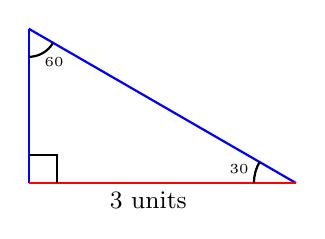
\begin{tikzpicture}
                \begin{axis}[
                    xmin = -10, xmax = 100,
                    ymin = -10, ymax = 100,
                    height = 5.5cm, width = 5.5cm,
                    axis lines = none%
                ]
                    %Triangle
                    \draw[color = blue, thick] (0,0) -- (0,55);
                    \draw[color = blue, thick] (0,55) -- ({55 / tan(30)}, 0);
                    \draw[color = red, thick] (0,0) -- ({55 / tan(30)}, 0);

                % 30 Degree Angle
                \node[font = \tiny] at (75, 5) {$30\degree$};
                \draw[color = black, thick] ({(55 / tan(30)) - 15},0) arc (180:150:15);

                % 60 Degree Angle
                \node[font = \tiny] at (9,43) {$60\degree$};
                \draw[color = black, thick] (0, {55-10}) arc (270:330:10);

                %Side Labels
                \node[font = \small] at ({55 / (2 * tan(30)) - 5}, -6) {$3$ units};           % xsqrt(3) label

                % Right angle symbol
                \draw[thick, color = black] (0,10) -- (10,10) -- (10,0);
                \end{axis}
            \end{tikzpicture}
        \end{minipage}
        \begin{minipage}[c]{0.50\linewidth}
            Since we know from looking at Figure \ref{fig:30-60-90} that the longer leg is $x\sqrt{3}$ units long, we can actually solve for $x$ and find the value of the shorter leg and hypotenuse.
        \end{minipage}
    \end{center}
    Let's start by setting $x\sqrt{3}$ equal to $3$ and solving for $x$.
    \begin{align*}
        x\sqrt{3} &= 3 \\
        x &= \frac{3}{\sqrt{3}} \\
        x &= \frac{3\sqrt{3}}{3} \\
        x &= \sqrt{3}
    \end{align*}
    The $x$ we just found is the length of the shorter leg. Since the hypotenuse is known to be $2x$ in length, doubling this gives us the length of the hypotenuse.
    \begin{align*}
        \sqrt{3} \cdot 2 &= 2\sqrt{3}
    \end{align*}
    That gives us the triangle below.
    \begin{center}
        \centering
        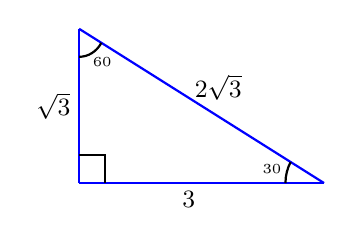
\begin{tikzpicture}
            \begin{axis}[
                xmin = -20, xmax = 100,
                ymin = -10, ymax = 100,
                height = 5.5cm, width = 5.5cm,
                axis lines = none%
            ]
                %Triangle
                \draw[color = blue, thick] (0,0) -- (0,55);
                \draw[color = blue, thick] (0,55) -- ({55 / tan(30)}, 0);
                \draw[color = blue, thick] (0,0) -- ({55 / tan(30)}, 0);

            % 30 Degree Angle
            \node[font = \tiny] at (75, 5) {$30\degree$};
            \draw[color = black, thick] ({(55 / tan(30)) - 15},0) arc (180:150:15);

            % 60 Degree Angle
            \node[font = \tiny] at (9,43) {$60\degree$};
            \draw[color = black, thick] (0, {55-10}) arc (270:330:10);

            %Side Labels
            \node[font = \small] at (-10, {55 / 2}) {$\sqrt{3}$};                         % x label 
            \node[font = \small] at ({55 / (2 * tan(30)) - 5}, -6) {$3$};                           % xsqrt(3) label
            \node[font = \small] at ({55 / (2 * tan(30)) + 6.5}, {(55 / 2) + 6.5}) {$2\sqrt{3}$};       % 2x label

            % Right angle symbol
            \draw[thick, color = black] (0,10) -- (10,10) -- (10,0);
            \end{axis}
        \end{tikzpicture}
    \end{center}
\end{solution}
\begin{problem}
    Given an isosceles right triangle with a hypotenuse of $4$ units, find the length of its two legs.
\end{problem}
\begin{solution}
    Let's look at what we're given.
    \begin{enumerate}
        \item We're given that this is a right triangle, meaning it must have one angle of $90\degree$.
        \item We're given that the hypotenuse of this triangle is $4$ units.
        \item We're given that this triangle is not only a right triangle, but an isosceles triangle. This means that the two legs are the same length.
    \end{enumerate}
    \clearpage
    With the given information, we can see that we're working with a 45-45-90 triangle. We have a $90\degree$ angle and two sides that are the same length. That exactly matches the two legs of length $x$ seen in Figure \ref{fig:45-45-90}. Also from that figure, recall that the hypotenuse has a length of $x\sqrt{2}$ units.

    With that, we can set $x\sqrt{2}$ equal to $4$ and solve for $x$.
    \begin{align*}
        x\sqrt{2} &= 4 \\
        x &= \frac{4}{\sqrt{2}} \\
        &= \frac{4\sqrt{2}}{2} \\
        &= 2\sqrt{2}
    \end{align*}
    The $x$ we just solved for is the length of both legs (since they're the same length). That also means we're done.
    \begin{center}
        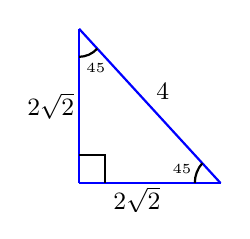
\begin{tikzpicture}
            \begin{axis}[
                xmin = -20, xmax = 100,
                ymin = -10, ymax = 100,
                height = 5.5cm, width = 5.5cm,
                axis lines = none%
            ]
            %Triangle
            \draw[color = blue, thick] (0,0) -- (0,55);
            \draw[color = blue, thick] (0,55) -- ({55 / tan(45)}, 0);
            \draw[color = blue, thick] (0,0) -- ({55 / tan(45)}, 0);

            % 30 Degree Angle
            \node[font = \tiny] at (40,5) {$45\degree$};
            \draw[color = black, thick] ({(55 / tan(45)) - 10},0) arc (180:135:10);

            % 60 Degree Angle
            \node[font = \tiny] at (6.5,41) {$45\degree$};
            \draw[color = black, thick] (0, {55-10}) arc (270:315:10);

            %Side Labels
            \node[font = \small] at (-11, {55 / 2}) {$2\sqrt{2}$};                                       % x label 
            \node[font = \small] at ({55 / (2 * tan(45)) - 5}, -6) {$2\sqrt{2}$};                       % xsqrt(3) label
            \node[font = \small] at ({55 / (2 * tan(45)) + 5}, {(55 / 2) + 5}) {$4$};   % 2x label

            % Right angle symbol
            \draw[thick, color = black] (0,10) -- (10,10) -- (10,0);
            \end{axis}
        \end{tikzpicture}
    \end{center}
\end{solution}
Let's look at one last problem that's a bit different from the rest before continuing. As always, I encourage you to try the problem yourself before looking at the solution.
\begin{problem}
    Determine the type of special triangle that has side lengths of $3$, $4$, and $5$ units.
\end{problem}
\begin{solution}
    The two types of special triangles we've covered are the 30-60-90 and the 45-45-90. First and foremost, let's confirm whether this triangle is even a right triangle.

    To do this, we'll use the Pythagorean Theorem ($a^2 + b^2 = c^2$). If this equation holds, then we can continue to the next step.
    \clearpage
    I'll define $a = 3$, $b = 4$, and $c = 5$. The order of $a$ and $b$ do not matter because they are the legs. However, $c$ \textbf{must} be $5$. The length of $5$ units is the longest of the three, so it \textbf{must} be the hypotenuse.

    Substituting those values in gives:
    \begin{align*}
        3^2 + 4^2 &= 5^2 \\
        9 + 16 &= 25 \\
        25 &= 25
    \end{align*}
    The Pythagorean Theorem holds, so we've confirmed that this triangle is a right triangle and can continue to the next part of the solution.

    First, let's test to see if this is a 30-60-90 triangle. Recall that the short leg has a length of $x$, the long leg has a length of $x\sqrt{3}$, and the hypotenuse has a length of $2x$.

    In the given triangle, the short leg ($x$) is $3$, the long leg is $4$, and the hypotenuse is $5$. That means:
    \begin{itemize}
        \item $x = 3$
        \item $x\sqrt{3} = 4$
        \item $2x = 5$
    \end{itemize}
    Since we're already given that $x = 3$, let's try plugging that into the other two equations.
    \begin{align*}
        3\sqrt{3} \neq 4 \qquad 2(3) = 6 \neq 5
    \end{align*}
    Since a value of $x = 3$ doesn't make sense given the side lengths, we can say that this is not a 30-60-90 triangle.

    Now, let's see whether this is a 45-45-90 triangle. Same as before, we'll state the side lengths.
    \begin{itemize}
        \item $x = 3$ (leg 1)
        \item $x = 4$ (leg 2)
        \item $x\sqrt{2} = 5$ (hypotenuse)
    \end{itemize}
    This fails immediately. We have an $x = 3$ \textbf{and} and $x = 4$. Therefore, this is also not a 45-45-90 triangle.

    This was actually a trick question. The triangle described isn't a special triangle at all. It's actually what's referred to as a \textbf{Pythagorean Triple}, meaning all three sides are integers and form a right triangle.

    Other examples of Pythagorean Triples are the 8-15-17 and 12-35-37. However, the 3-4-5 triple is most commonly used.
\end{solution}